%! Author = t.kramer
%! Date = 10/06/2023

\section{Case study}

We conducted the case study with the aim of testing the implementation of the proposed framework in \textit{comfortSIM}. We sought to examine the effect of various \gls{ml} algorithms on the performance of the prediction model, to investigate the potential of using \gls{pcs} to enhance \gls{sta} and reduce the required energy use, and evaluate projected personal and spatial variations in thermal comfort for the featured cases.


\begin{figure*}[!h]
    \begin{center}
    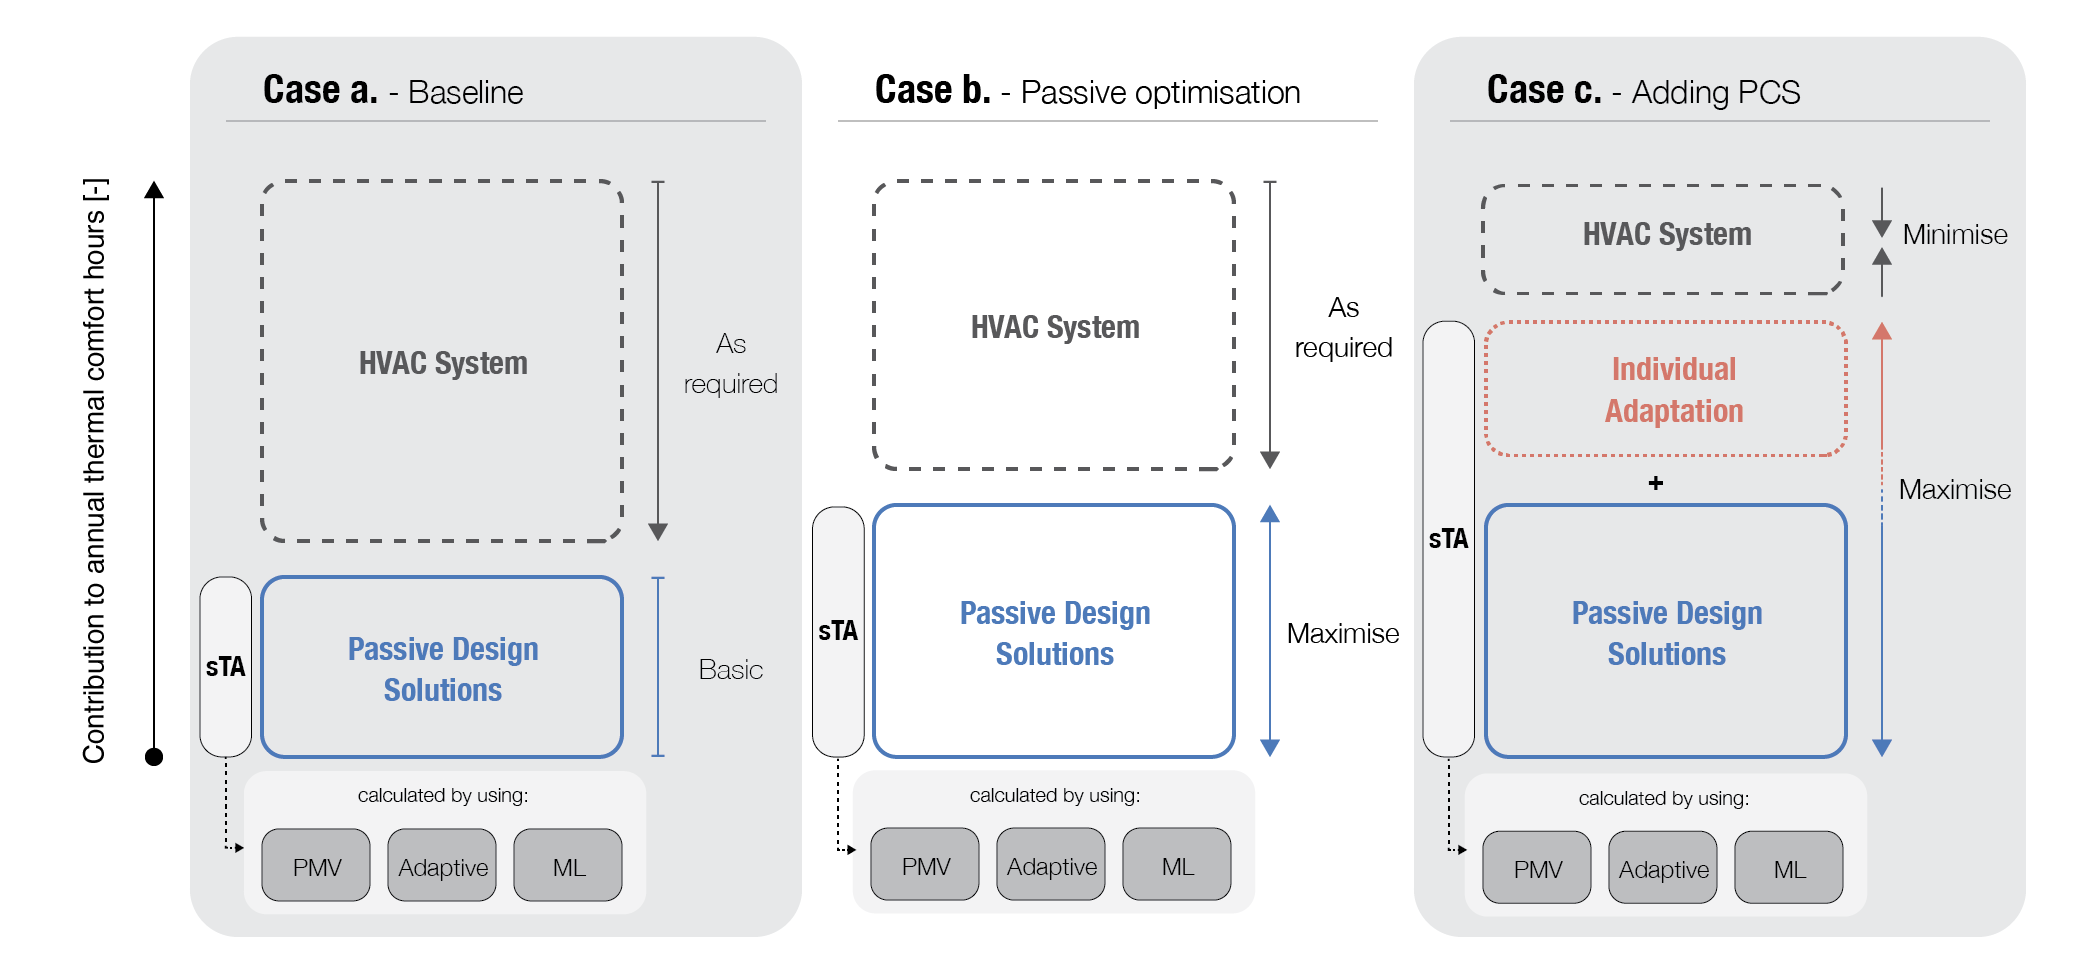
\includegraphics[width=\textwidth]{manuscript/src/figures/case-study-concept.png}
    \caption{Case study simulation concept: The aim was to test a reference building for three specific scenarios: (a) a baseline case where the building model is predominantly conditioned by an \gls{hvac} system; (b) a mixed-mode case with more focus on passive design optimisation; and (c) the additional use of \gls{pcs} (compared to (b)).}
    \label{fig:case-study-concept}
    \end{center}
\end{figure*}


As a baseline scenario, we created a reference office building simulation model using standard settings for constructions, internal loads, and schedules provided by the U.S. Department of Energy (DOE). The created model was simulated for an entire year and the climate of Brisbane, Australia (Cfa). We used the combination of Rhinoceros, Grasshopper and Ladybug Tools to model and simulate the test building. The Honeybee library included in Ladybug Tools is built on EnergyPlus. Here, we used the spatial climate mapping algorithm \citep{Mackey2015} discussed earlier to calculate the indoor environmental parameters of air temperature, relative humidity, and mean radiant temperature on a 1 m by 1 m grid. This resulted in a simulation grid of 405 points for the 500 \si{\square\metre} building model.

For each scenario summarised in \Cref{fig:case-study-concept}, we first simulated an unconditioned scenario to calculate \gls{sta}. More information on the building model and simulation settings is provided in \Cref{tab:sim-settings}. In addition, the IDF simulation file will be made available on GitHub for reference.



\begin{figure}[!h]
    \centering
    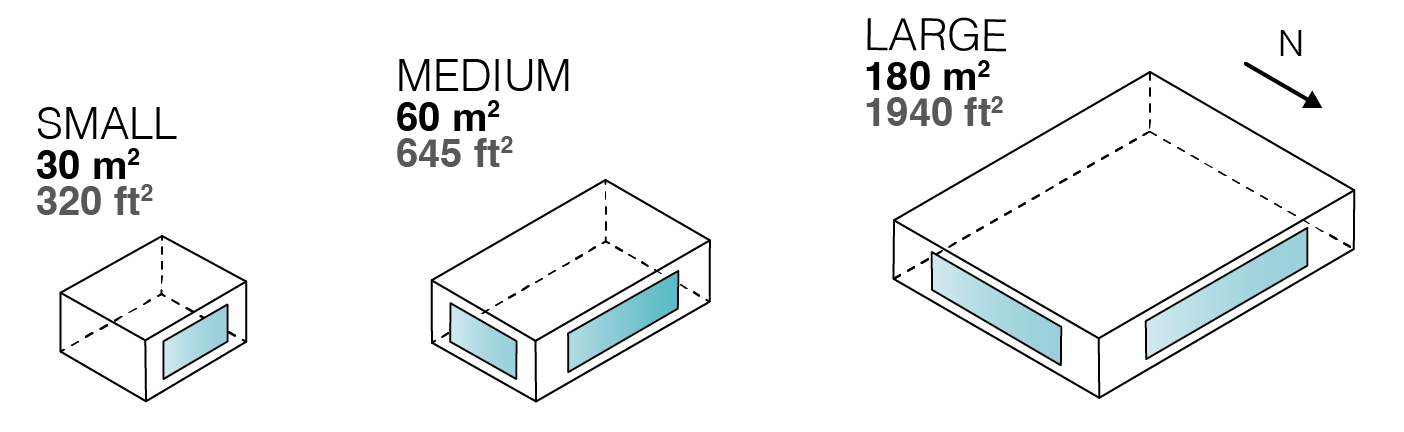
\includegraphics[width=0.8\textwidth]{manuscript/src/figures/scenario-size.png}
    \vspace{0.5cm}
    % \caption{Geometry of case study model.}

        \renewcommand{\arraystretch}{1.25}
    

        \begin{tabular}{ p{3.5cm} p{2cm} p{2cm} p{2cm} }
        
            \hline
            
            {\textbf{Setting(s)}} & \multicolumn{3}{l}{\textbf{Definition}} \\
        
            \hline
        
            {Climates}  & \multicolumn{3}{l}{Sydney, Australia (Cfa), TMY \& 2070 (RCP 4.5)} \\
        
            % \cline{2-3}
            
            {Constructions} & \multicolumn{3}{l}{\textit{ASHRAE 90.1 2019, IECC 2021}, Steel-framed*} \\
        
            % \cline{2-3}  
            
            {Program} & \multicolumn{3}{l}{\textit{Small Office*}} \\
            
            % \cline{2-3}
        
            {HVAC system} & \multicolumn{3}{l}{IdealAir system, Air conditioned} \\
        
            % \cline{2-3}

            {Passive Design Level} & {a) \textbf{Standard}} & {b) \textbf{Medium}} & {c) \textbf{Advanced}} \\

            \cline{2-4}
        
            {Natural Ventilation?} & {No} & {Yes} & {Yes} \\
        

            {Envelope} & {$U_{win} = 2.0$\newline $U_{wall} = 0.35$\newline $WWR = 0.4$ \newline No shading} & {$U_{win} = 1.3$\newline $U_{wall} = 0.2$\newline $WWR = 0.3$ \newline No shading} & {$U_{win} = 1.3$\newline $U_{wall} = 0.2$\newline $WWR = 0.3$ \newline Ext. shading} \\

             % \cline{2-3}
        
            {AC* setpoint range\newline \textit{Heating - Cooling}} & {22-24\degree C} & {22-24\degree C} & {22-24\degree C} \\
            
            \hline
        
        \end{tabular}
        \vspace{0.5cm}
        \caption{Overview of main settings for simulated case study scenarios: Construction properties, loads and schedules were based on Department of Energy (DOE) reference building information. (AC* - Air Conditioning (if used), WWR - Window-to-Wall-Ratio, U - U value in W/m²K)}
        \label{tab:sim-settings}
        

\end{figure}

%%%%%%%%%%%%%%%%%%%%%%%%%%%%%%%%%%%%%%%%%%%%%%%%%%%

\subsection{Thermal preference prediction model performance}
\label{sec:results-ml}

We evaluated the performance of different \gls{ml} algorithms for the prediction model. The performance of the algorithms was initially optimised on the training dataset using the common \textit{GridSearch} and \textit{k-fold cross validation} methods in Scikit-learn \citep{Pedregosa2011}. For simplicity and transparency, we selected \gls{logr} as the baseline algorithm. Furthermore, we tested a \gls{svc} and a Decision Tree method (\gls{rf}) as well as a stacking classifier combining \gls{logr} and \gls{rf}.

In addition to the main metrics of \textit{Recall}  and \textit{ROC-AUC}, we compared the prediction time for each classifier. The 405 grid points multiplied by 8760 annual simulation hours yielded more than 3.5 million rows of predicted target variables, so the prediction time is not insignificant and influences the feasibility of using the model in practise.

We then compared the results for all algorithms tested with similar data for the \gls{pmv} model, as a representation of conventional thermal comfort models, and calculated using the pythermalcomfort package \citep{TartariniPythermalComfort2020} in Python.


\begin{figure*}[!h]
    \begin{center}
    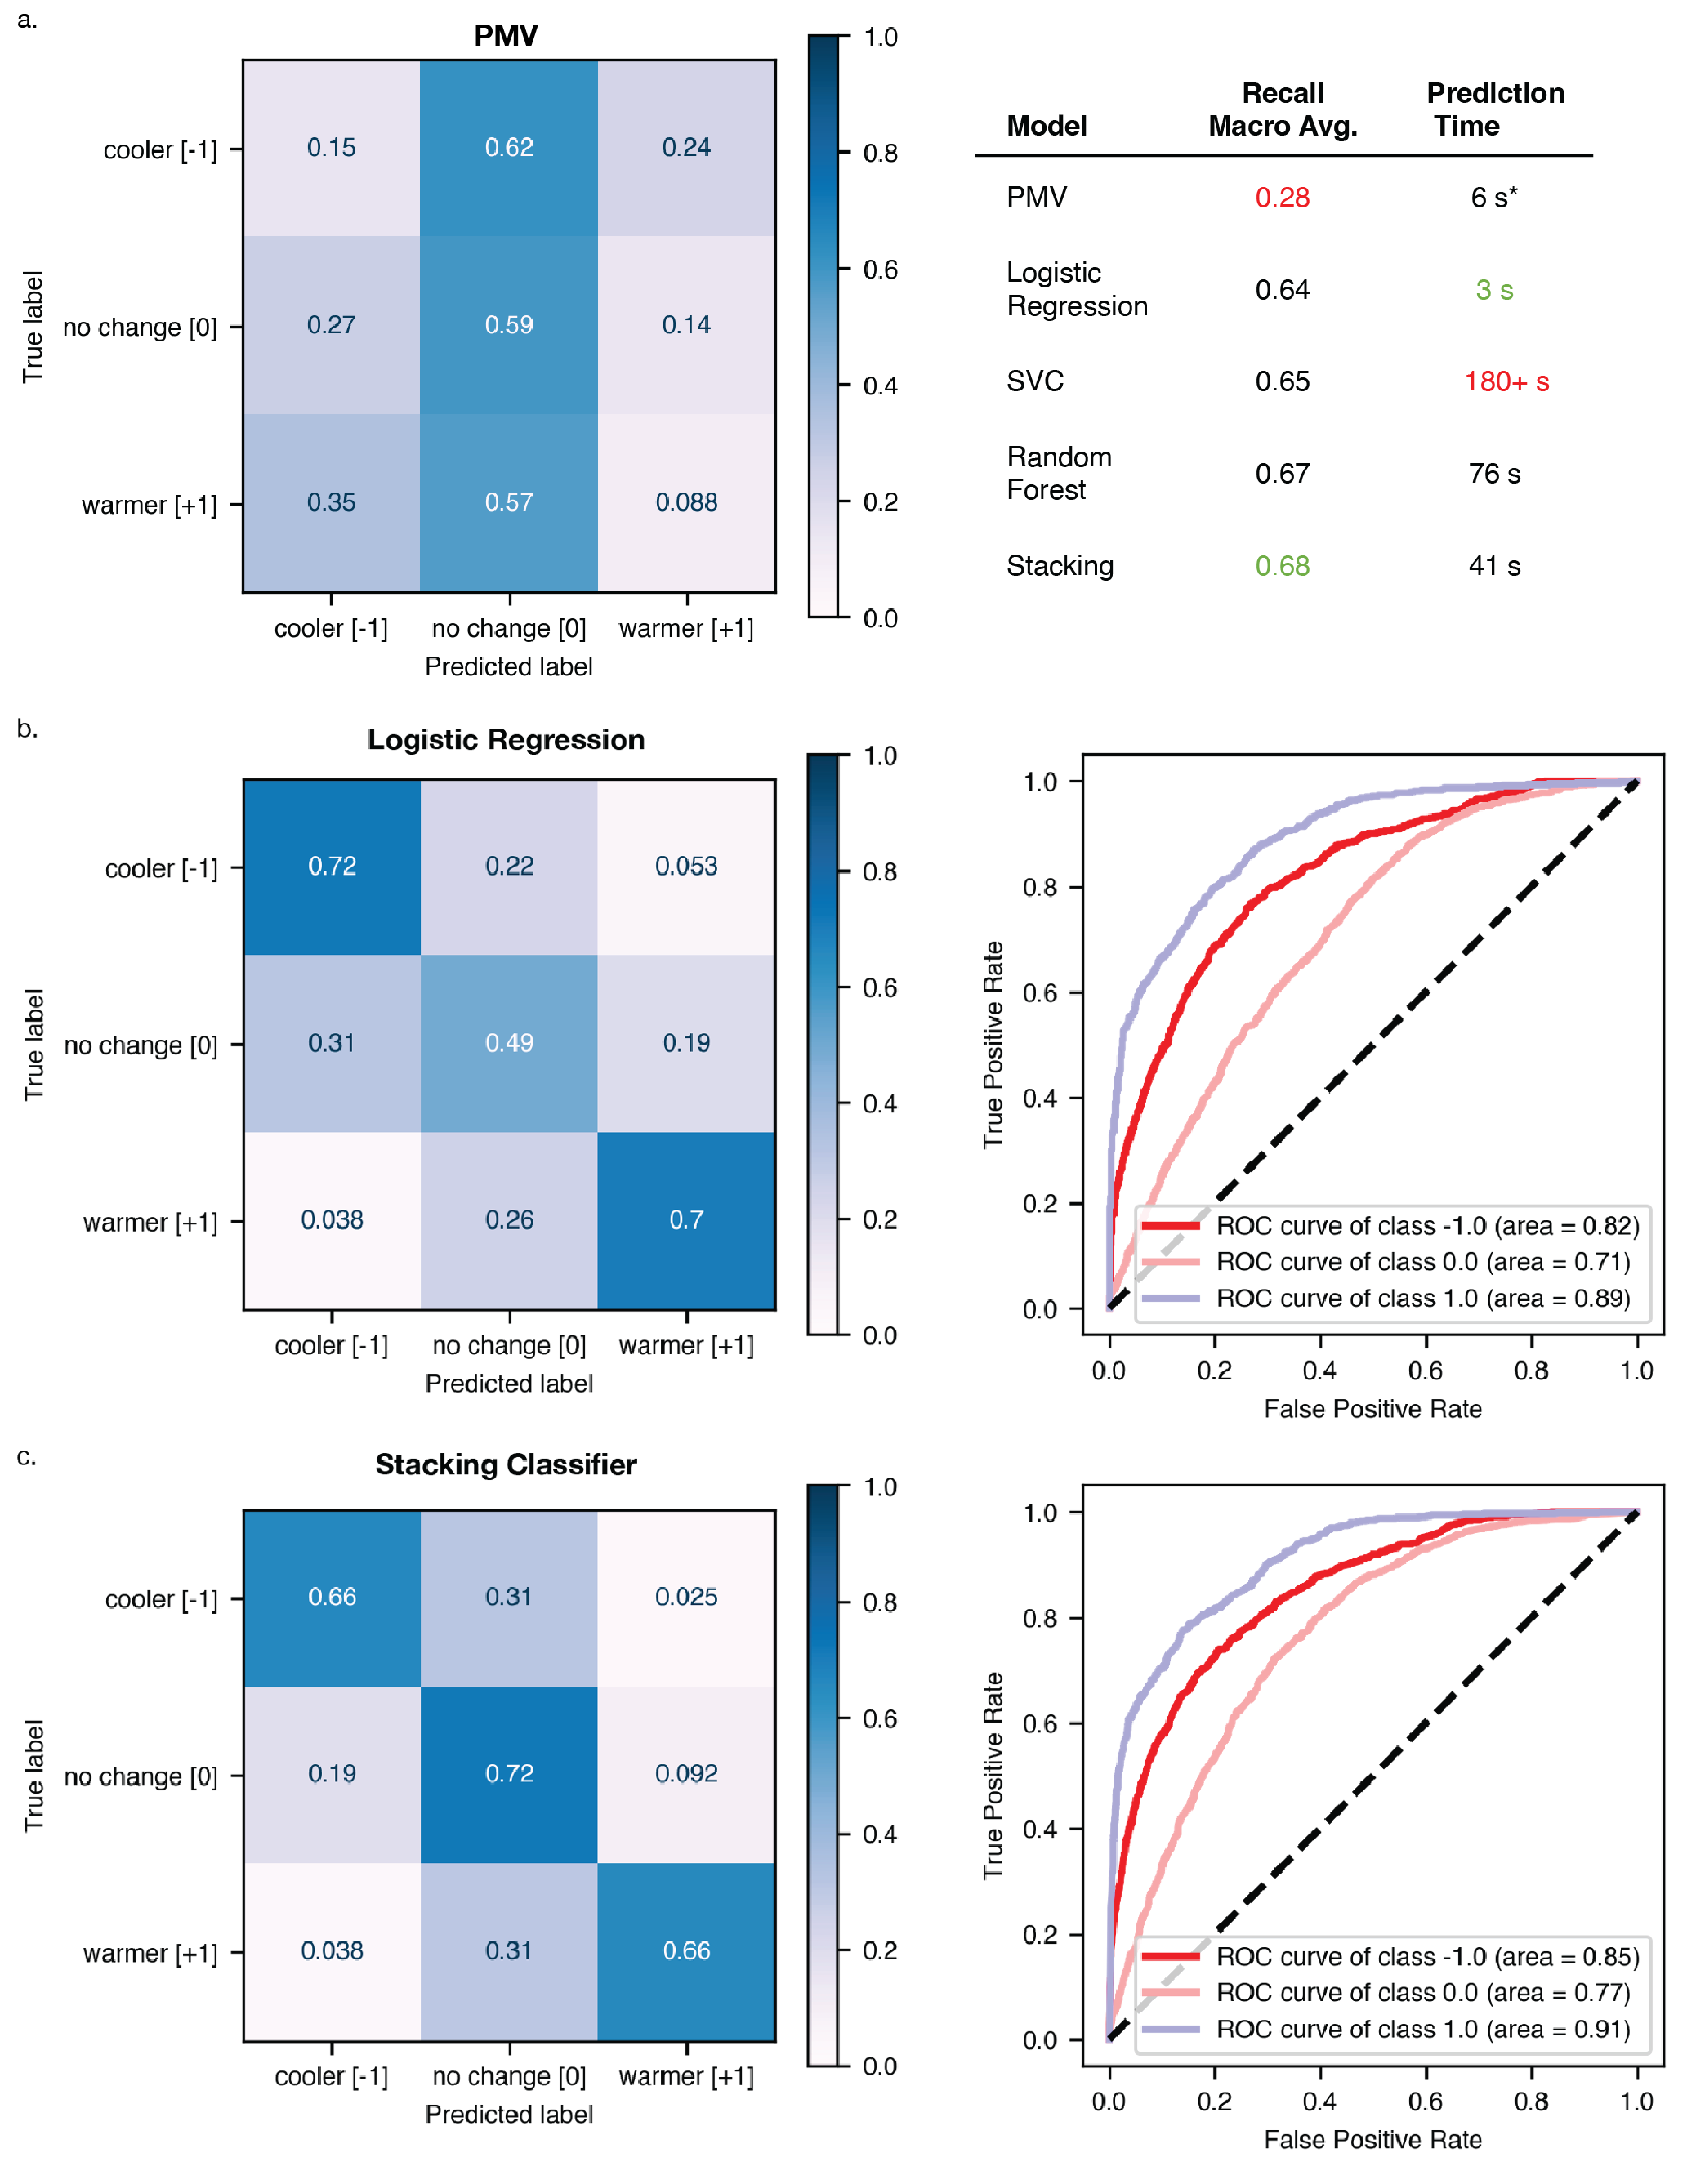
\includegraphics[width=\textwidth]{manuscript/src/figures/roc-auc.png}
    \caption{Performance of tested ML Thermal Preference classifiers: \gls{pmv} was converted to thermal preference using $|PMV| \le 0.5$ = ‘no change’ [0]; $PMV > 0.5$ = ‘cooler [-1]’; and $PMV <$ -0.5 = ‘warmer’ [+1] as in \citep{KimZhou2018}.}
    \label{fig:jp-iii-roc-auc}
    \end{center}
\end{figure*}


The results shown in \Cref{fig:jp-iii-roc-auc} demonstrate that the \gls{ml} classifiers outperformed the \gls{pmv} model in terms of accuracy for the positive classes of 'cooler' (-1) and 'warmer' (+1). This is evident from the confusion matrices on the left side of subplots \Cref{fig:jp-iii-roc-auc}.a-c. In contrast, the \gls{pmv} model has considerably lower accuracy for the more important positive classes and tends to predict 'No change' (0) in the majority of cases. This results in a relatively low recall value of 0.28 for the \gls{pmv} method.

A comparison of the \gls{ml} algorithms reveals that the stacking classifier (\gls{logr} \& \gls{rf}) achieves the highest recall value of 0.68, which is slightly more precise than the \gls{logr} (0.64). This is consolidated by the Area under the ROC Curve (AUC) values, which demonstrate the better overall prediction performance of the stacked algorithm.

When incorporating \gls{ml} algorithms into building performance simulations, the prediction time is a significant factor. The \gls{logr} classifier had the lowest prediction time, closely followed by \gls{pmv} Python implementation. On the other hand, Stacking, \gls{rf} and \gls{svc} took much longer to predict on the test dataset. This is evident from the table in the upper right corner of \Cref{fig:jp-iii-roc-auc}.

Based on solid prediction performance and the shortest overall prediction time, we chose the \gls{logr} classifier for implementation in the building performance simulation workflow in the rest of the case study.


%%%%%%%%%%%%%%%%%%%%%%%%%%%%%%%%%%%%%%%%%%%%%%%%%%%

\subsection{sTA and energy use}

A main objective of this pilot study was to test the \textit{comfortSIM} method and to investigate the connections between \gls{sta}, thermal comfort models used and the projected energy use for the evaluated building model.


\begin{figure*}[!h]
    \begin{center}
    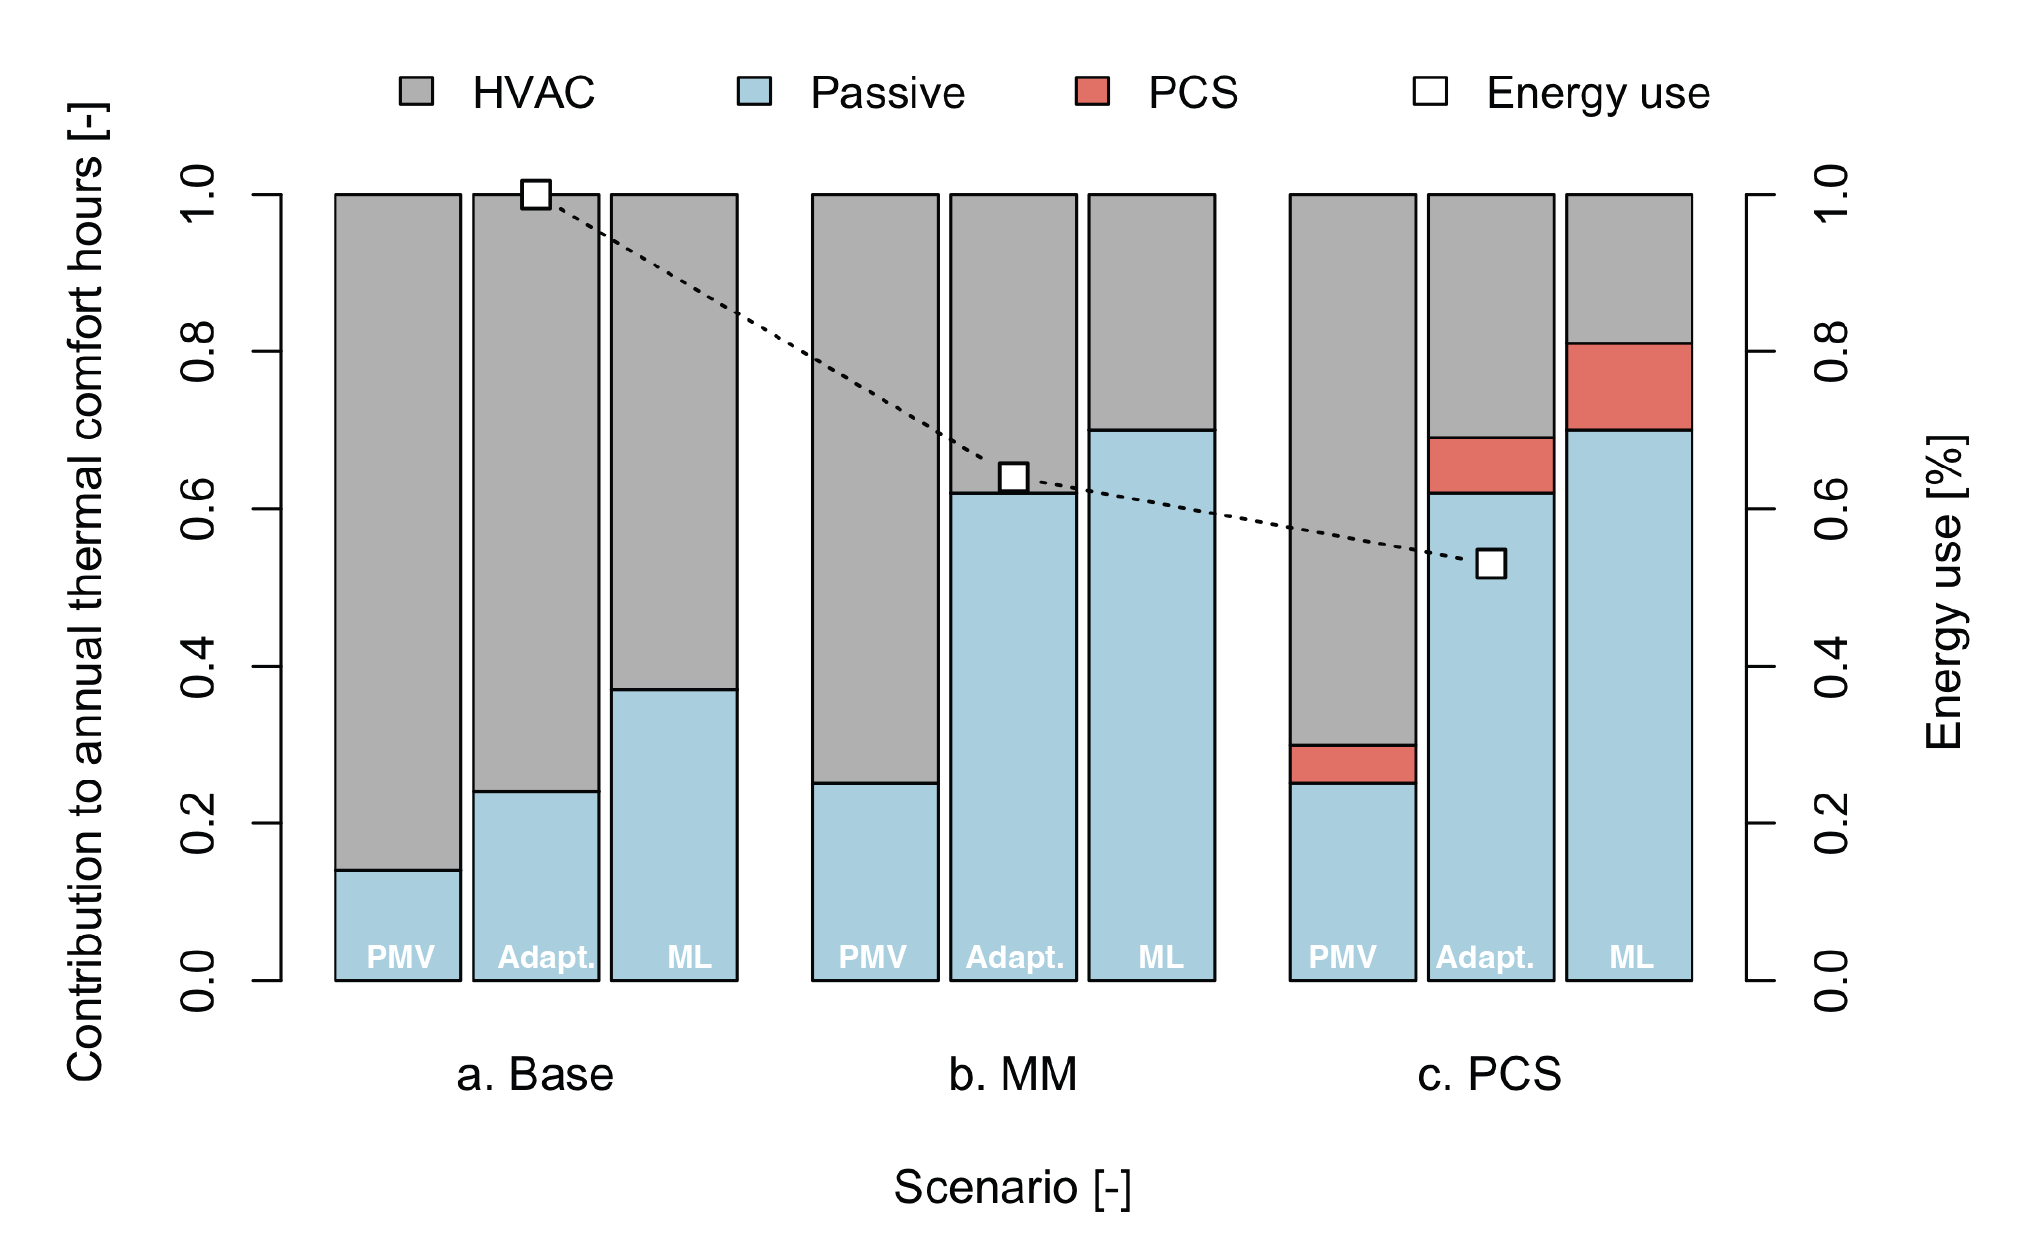
\includegraphics[width=\textwidth]{manuscript/src/figures/sta-comfort-hour-contribution.png}
    \caption{Projected contribution of \gls{hvac} system, passive building design and personal adaptation through \gls{pcs} to annual thermal comfort hours and the influence of their composition on energy use for the investigated cases. Spatial Thermal Autonomy (sTA) was calculated using three different thermal comfort models, the \gls{pmv}, the adaptive model, and the trained \gls{ml} classifier and equals the sum of the contributions by passive design strategies and \gls{pcs}: PCS contribute to an improvement of \gls{sta} and a reduction in energy use for all tested models.}
    \label{fig:sta-comfort-hours}
    \end{center}
\end{figure*}


\gls{sta} measures how successful a building is expected to be in providing passive thermal comfort. Initially, we examined the influence of building design and conditioning strategies on \gls{sta} for each simulated scenario. Here, \Cref{fig:sta-comfort-hours} reveals a clear trend that the implementation of passive design solutions (b \& c) resulted in significantly higher \gls{sta} than the baseline scenario (a). This emphasises the importance of passive design solutions and the combined effect of architectural and conditioning decisions in optimising thermal autonomy and performance.

By comparing cases (a) and (b), it is also evident that this improvement in \gls{sta} (+ 37\%) corresponds to considerable energy savings of up to 36\%.

Furthermore, \Cref{fig:sta-comfort-hours} highlights the impact of using \gls{pcs} on reducing energy use and improving \gls{sta}. For all models studied, it can be seen that using \gls{pcs} in the operational phase of the building can result in \gls{sta} improvements of up to 11\%. This means that using \gls{pcs} in a temperate climate such as Brisbane, the time in thermal comfort without using energy for conditioning can be increased by more than two hundred hours. This translates into at least five additional working weeks of autonomy from energy-intensive \gls{hvac} systems. For the investigated case, and averaged for all thermal comfort models tested, the corresponding energy savings amount to 10\%.

Focusing on the effect of the chosen comfort model on the resulting \gls{sta}, it is noteworthy that the \gls{pmv} model resulted in significantly lower \gls{sta} values. For each situation, the \gls{pmv}-based \gls{sta} is less than half of what the \gls{ml} is forecasting. The difference between \gls{pmv} and Adaptive model is similar, particularly for cases (b) and (c). Together, these observations emphasise that the Adaptive Model and the \gls{ml} classifer, both based on extensive \gls{poe} data from real buildings, encourage wider comfort ranges and less reliance on energy for space conditioning.


%%%%%%%%%%%%%%%%%%%%%%%%%%%%%%%%%%%%%%%%%%%%%%%%%%%

\subsection{Personal and spatial diversity}

Using the derived thermal sensation offset classes as a feature for the thermal preference classifier allowed us to test the projected thermal preference in the simulated conditions for each offset class. \Cref{fig:diversity}.a compares the annual distribution of predicted thermal preferences between offset classes before and after applying the proposed \gls{pcs} algorithm.


\begin{figure*}[!h]
    \begin{center}
    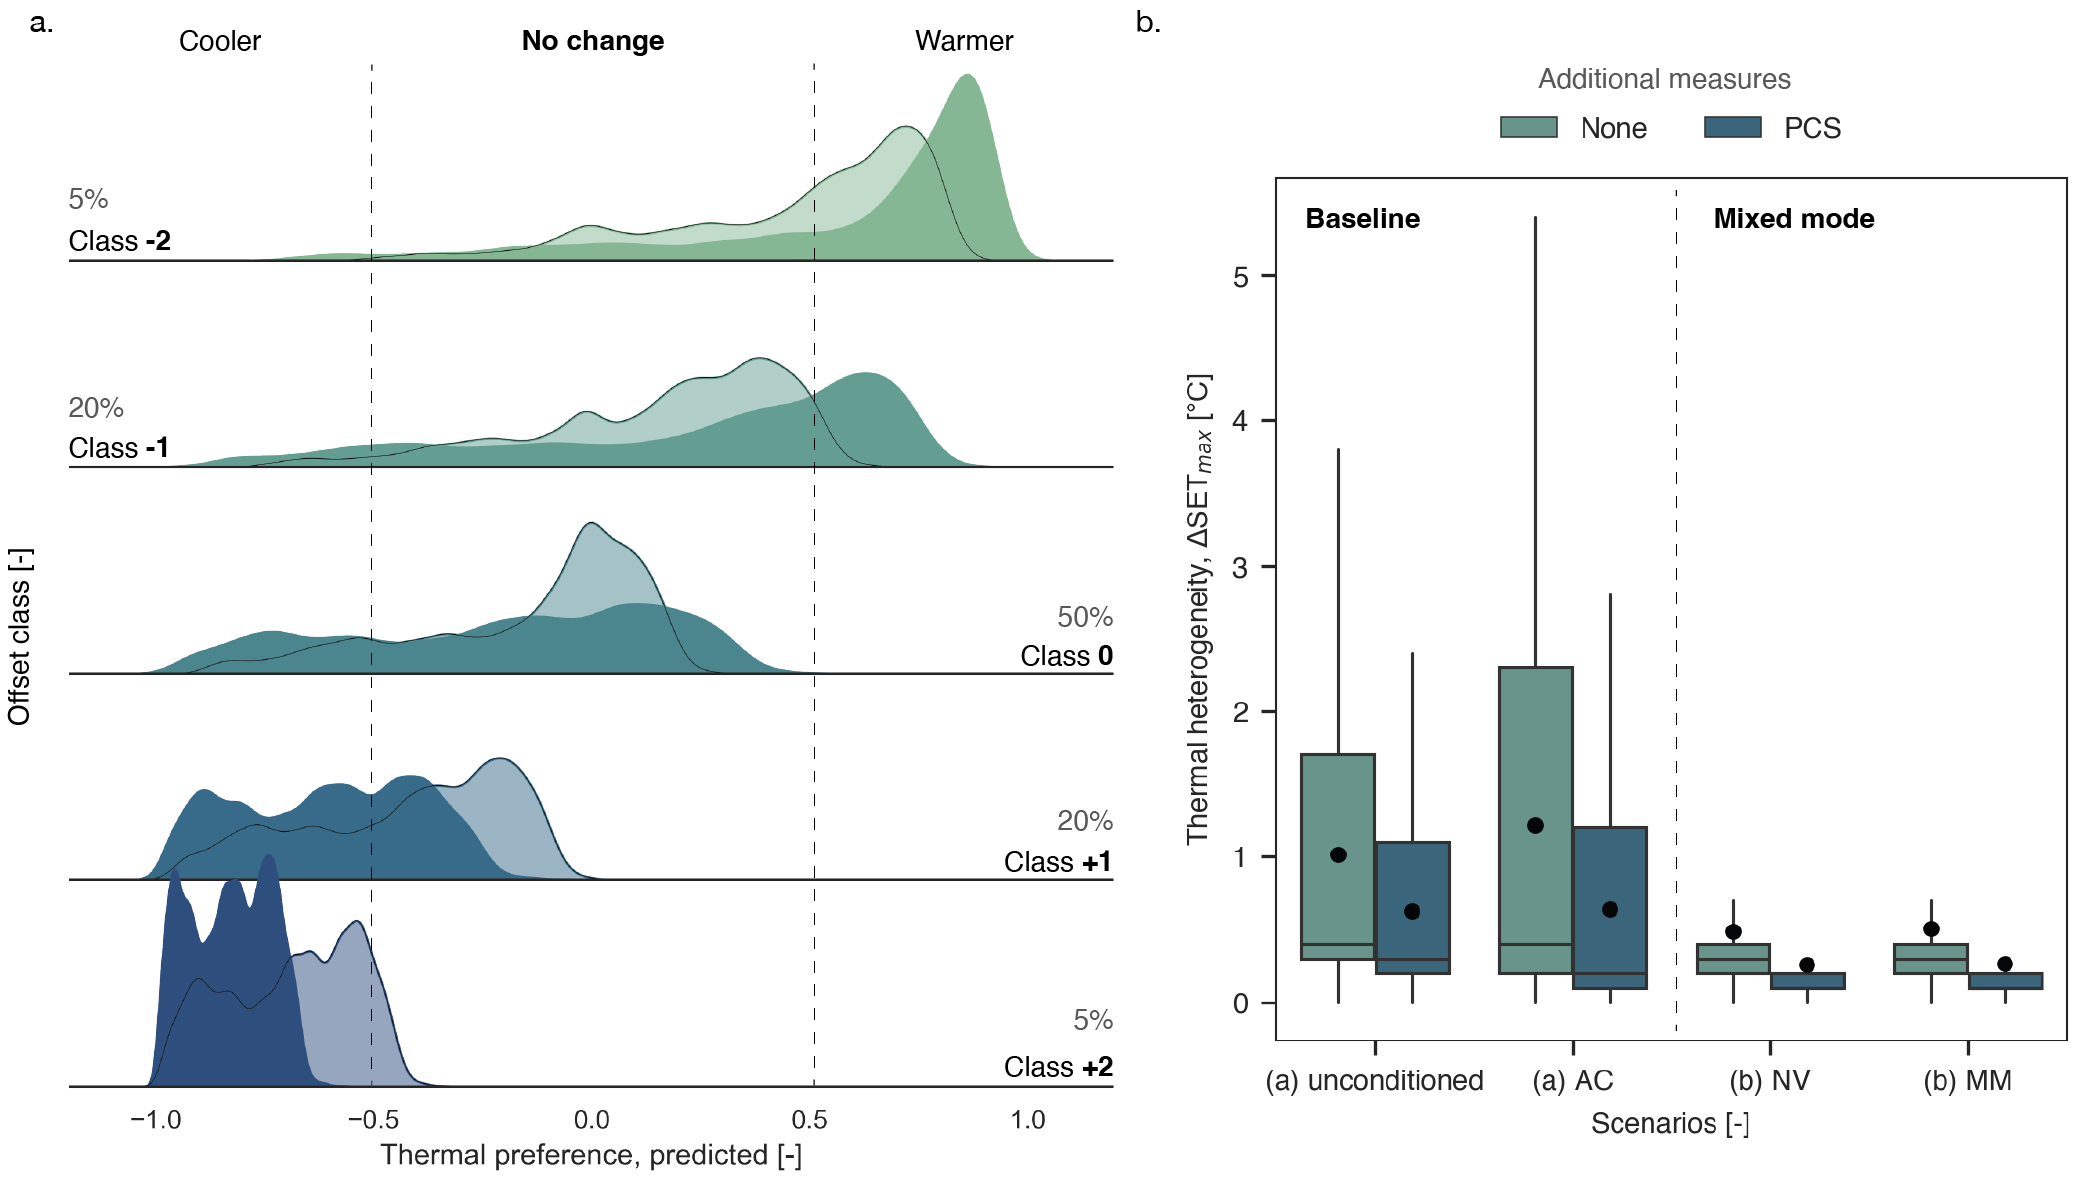
\includegraphics[width=\textwidth]{manuscript/src/figures/personal-spatial-diversity.png}
    \caption{Overview of predicted diversity in thermal preference and spatial thermal conditions: a.) Predicted annual thermal preference distribution of each personal offset class and potential effect of providing \gls{pcs} for thermal adaptation; b.) Predicted $\Delta SET_{max}$ for Cases (a) and (b) and effect of \gls{pcs} on anticipated spatial thermal heterogeneity (both Case (a) and Case (b) were evaluated for both the unconditioned and (partially) conditioned scenario). }
    \label{fig:diversity}
    \end{center}
\end{figure*}


The figure highlights the positive effect of providing adaptive opportunity through \gls{pcs}. For all classes, using \gls{pcs} leads to a shift of the thermal preference spectrum to the "No change" range, indicating that the heating and cooling effect of \gls{pcs} helps alleviate discomfort and action thermal preferences. However, the effect is different for the five offset classes. \gls{pcs} seem to be more successful for the mid-range classes (-1, 0 and +1) where a large share of the initially uncomfortable predictions can be shifted to the "No change" range.

\Cref{fig:diversity}.a reveals a considerably wide range of thermal preference between classes. First, it is evident that occupants in classes -1, 0 and +1 are more likely to prefer "No change" in thermal conditions, especially when provided with \gls{pcs}. However, it can also be seen that occupants classified into classes -2 and +2 tend to prefer a change in thermal conditions, even after providing an opportunity for personal adaptation via \gls{pcs}. While the share of occupants assigned to these border classes is low in comparison (analysis of the ASHRAE Global Thermal Comfort Database II suggests less than 10\% for each group (see \Cref{sec:classification})), the generally wide range of predicted thermal preferences emphasises the need to provide adaptive opportunity for these persona types.

Another aspect covered in \Cref{fig:diversity}.b is the effect of passive design measures and \gls{pcs} on spatial thermal diversity. The box plot compares the annual distribution of $\Delta SET_{max}$ for cases (a) and (b) with the alternate scenario of adding \gls{pcs} in each case. The box plot shows that \gls{pcs} can be a valuable tool not only to improve personal thermal comfort, but also to reduce spatial thermal heterogeneity in a space. First, it is evident that the implementation of passive strategies (difference between scenarios (a) and (b)) can significantly reduce spatial heterogeneity. This is underlined by the decrease in mean values and the significantly narrower ranges of the simulated $\Delta SET_{max}$. Second, for all tested cases, providing and applying \gls{pcs} based on personal preferences significantly reduces spatial heterogeneity within the space. For each scenario, the use of \gls{pcs} leads to a reduction in the mean value and the overall range of thermal diversity represented by $\Delta SET_{max}$. Even for a passively well-designed building, as denoted in case (b), \gls{pcs} can lead to more homogeneous indoor thermal environments.

% In summary, \Cref{fig:diversity} emphasises that \gls{pcs} can be a valuable tool in providing opportunities for personal adaptation and reducing thermal heterogeneity in dynamic indoor environments.